\documentclass[pra,12pt]{revtex4}
\usepackage{amsmath}
\usepackage{amssymb}
\usepackage{graphicx}
\usepackage{color}
\usepackage{mathrsfs}
\usepackage{enumerate}
\usepackage{framed}
\usepackage[pdfborder={0 0 0},colorlinks=true,linkcolor=blue,urlcolor=blue]{hyperref}

\def\ket#1{\left|#1\right\rangle}
\def\bra#1{\left\langle#1\right|}
\def\braket#1{\left\langle#1\right\rangle}

\usepackage{fancyhdr}
\fancyhf{}
\lhead{\tiny Y.~D.~Chong}
\rhead{\scriptsize PH4401: Quantum Mechanics III}
\lfoot{}
\rfoot{\thepage}
\pagestyle{fancy}

\setlength{\parindent}{14pt}
\renewcommand{\theequation}{1.\arabic{equation}}

\renewcommand{\baselinestretch}{1.0}
\setlength{\parskip}{0.07in}

\begin{document}

\begin{center}
{\Large \textbf{Chapter 1: Resonances}}
\end{center}

\section{Bound states and free states}

A curious feature of wavefunctions in infinite space is that they come
in two distinct varieties: (i) \textbf{bound states} that are
localized to one region of space, like the ground state of a harmonic
oscillator, and (ii) \textbf{free states} that extend over the whole
space, like plane waves.  In fact, both kinds of states can co-exist
in a single system.

A simple model exhibiting this is the \textbf{1D finite square well}.
Consider the Hamiltonian
\begin{equation}
  \hat{H} = \frac{\hat{p}^2}{2m} - U \,\Theta(a -|\hat{x}|),
\end{equation}
where $\hat{x}$ and $\hat{p}$ are 1D position and momentum operators,
$m$ is the particle mass, $U$ and $a$ are positive real parameters
governing the potential function, and $\Theta$ denotes the Heaviside
step function (i.e., 1 if the input is positive, and 0 otherwise).  As
shown below, the potential forms a well of depth $U$ and width $2a$,
and vanishes elsewhere.

\begin{figure}[h]
  \centering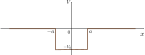
\includegraphics[width=0.55\textwidth]{squarewell}
\end{figure}

For such a Hamiltonian, the time-independent Schr\"odinger wave
equation can be solved efficiently using a technique called the
\textbf{transfer matrix method}.  Here, we will describe a few key
aspects of the calculation, bypassing most of the details.  For a more
detailed discussion of the transfer matrix method, refer to Appendix
B.

We begin by noting that deriving solutions to the Schr\"odinger wave
equation, like any other differential equation, requires us to specify
boundary conditions.

If we are interested in bound state solutions, we look for
wavefunctions that diminish exponentially as $x \rightarrow
\pm\infty$.  For $|x| > a$, the Schr\"odinger wave equation reduces to
\begin{equation}
  -\frac{\hbar^2}{2m}\,\frac{d^2\psi}{dx^2} = E \psi(x),
  \label{eq:psioutside}
\end{equation}
subject to the boundary conditions
\begin{equation}
  \psi(x) \sim e^{\mp\kappa x} \;\; \textrm{as} \;\; x \rightarrow \pm \infty
  \label{eq:expout}
\end{equation}
for some real $\kappa$.  The functions satisfying
Eqs.~\eqref{eq:psioutside} and \eqref{eq:expout} are
\begin{equation}
  \psi(x) = c_\pm\, e^{\mp\kappa x}, \;\;\mathrm{where}\;\, -\frac{\hbar^2\kappa^2}{2m} = E, \;\; c_\pm \in \mathbb{C}.
\end{equation}
Evidently, such a solution requires $E < 0$.  Moreover, the
variational principle implies that $E \ge -U$, so the bound state
energies are restricted to the range $-U \le E < 0$.

It is also possible to show that the bound state energies are
\textit{discrete}, and that each bound state wavefunction can always
be normalized:
\begin{equation}
  \int_{-\infty}^\infty |\psi(x)|^2\, dx\; =\; 1.
\end{equation}
The normalization integral is finite since $|\psi(x)|^2$ vanishes
exponentially for $x \rightarrow \pm \infty$.  These two properties
follow from the analysis of the general class of
``Sturm-Liouville-type'' differential equations; for details, refer to
textbooks such as Courant and Hilbert [\ref{cite:CourantHilbert}].

For a free state, the situation is quite different.  In this case, the
wavefunction does not vanish exponentially at infinity, but instead
takes the form
\begin{equation}
  \psi(x) = \begin{cases} \alpha_-\, e^{ik x} + \beta_-\, e^{-ik x}, & \;\;\;x < -a\\ (\mathrm{something}) , & -a < x < a\\ \alpha_+\, e^{ik x} + \beta_+\, e^{-ik x} , & \;\;\,x > a\end{cases}
\end{equation}
for some real $k$.  Right now, we are not concerned about how
$\psi(x)$ behaves in the well region $-a < x < a$.  We focus on the
outside region, where $\psi(x)$ consists of superpositions of
left-moving and right-moving plane waves.  To satisfy Schr\"odinger's
equation here, we need
\begin{equation}
  \frac{\hbar^2k^2}{2m} = E,
\end{equation}
which implies that $E \ge 0$.  For each $E$, the coefficients
$\alpha_\pm$ and $\beta_\pm$ are not independent, but are linked by a
linear relation (see Appendix B).  Unlike the bound states, the free
states are not discrete; there exist free states for \textit{every} $E
\ge 0$.

Moreover, since $|\psi(x)|^2$ does not diminish at infinity, the
integral $\int_{-\infty}^\infty |\psi(x)|^2\, dx$ is divergent, so
these wavefunctions cannot be normalized to unity.

The following figure shows numerically-obtained results for a square
well with $U = 30$ and $a=1$ (in units where $\hbar = m =1$).  The
energy spectrum is shown on the left side.  There exist five bound
states; their plots of $|\psi|^2$ versus $x$ are shown on the right
side.  These results were computed using the transfer matrix method
described in Appendix B.

\begin{figure}[h]
  \centering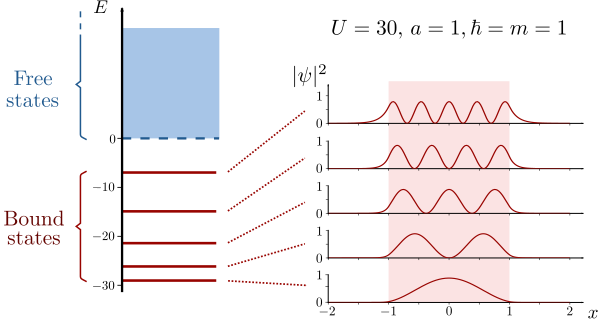
\includegraphics[width=0.76\textwidth]{boundvsextended}
\end{figure}

Many of the lessons drawn from the square well model can be
generalized to more complicated potentials.  In cases where the
potential at infinity is $V_{\textrm{ext}}$ rather than zero, free
states occur for $E \ge V_{\textrm{ext}}$ and bound states occur for
$\textrm{min}(V) < E < V_{\textrm{ext}}$.

There is an important proviso to bear in mind.  If we vary the
potential, the number of bound states can change: i.e., bound state
solutions can either appear or disappear.  A numerical example is
given below, showing the bound state energies for the square well
model with fixed $a = 1$, as we vary the potential minimum $-U$:

\vskip 0.15in
\begin{figure}[h]
  \centering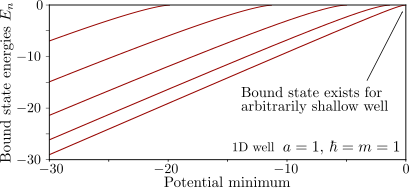
\includegraphics[width=0.71\textwidth]{boundstate1d}
\end{figure}

\noindent
For $U = 30$, there are five bound states, which disappear one by one
as we make the potential well shallower.  Note that one bound state
survives in the limit $U \rightarrow 0$.  There is a theorem stating
that any 1D attractive potential, no matter how weak, always supports
at least one bound state.  For details, see
\hyperref[ex:boundstate]{Exercise 1}.

In 3D, it is possible for an attractive potential to be too weak to
support a bound state.  Intuitively, this happens when the zero-point
energy of a prospective ground state exceeds the well depth.  The
figure below shows a numerical example, calculated for a uniform 3D
spherically symmetric well (the $l$'s labeling the various curves are
angular momentum quantum numbers).  To learn more about this
phenomenon, refer to \hyperref[ex:boundstate3d]{Exercise 2}.

\vskip 0.15in
\begin{figure}[h]
  \centering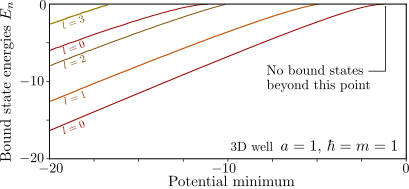
\includegraphics[width=0.71\textwidth]{boundstate3d}
\end{figure}

\clearpage

\section{Quasi-bound states and resonances}
\label{sec:resonances}

For the 1D finite square well, there is a clear distinction between
bound and free states.  Certain potentials, however, can host special
states called ``\textbf{quasi-bound states}''.  Like a bound state, a
quasi-bound state is strongly concentrated in one region of space, yet
it lies within the energy range of the free states continuum.  As we
shall see, quasi-bound states play an important important role in
scattering experiments.

The figure below shows an example of a potential function that gives
rise to quasi-bound states.  In the exterior region, $|x| > b$, the
potential is zero.  Between $x = -b$ and $x = b$, there is a
``barrier'' of positive potential $V_b$.  Embedded in the middle of
this barrier is a central well of depth $U$ and width $2a$, such that
$0 < V_b - U < V_b$.

\begin{figure}[h]
  \centering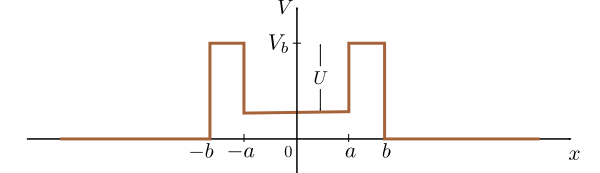
\includegraphics[width=0.65\textwidth]{resonancewell}
\end{figure}

\noindent
The potential is purely repulsive (i.e., $V \ge 0$ everywhere), so
there are no true bound states.  All the exact eigenstates of the
Hamiltonian must be free states.

However, there is something intriguing about the central well.
Consider an alternative scenario where the potential in the exterior
region is $V_b$ rather than $0$, so that
\begin{equation}
  V_{\mathrm{alt}}(x) = \begin{cases}V_b - U, & |x| < a, \\ V_b, & \mathrm{otherwise}.\end{cases}
\end{equation}
This describes a finite square well, which should have one or more
bound states in the energy range $V_b-U < E < V_b$.  For each of these
bound states, the wavefunction $\psi(x)$ diminishes exponentially away
from the well, so $\psi(x) \approx 0$ for $|x| > b$.  But $V(x)$ and
$V_{\mathrm{alt}}(x)$ differ only in the region $|x| > b$, which
implies that $\psi(x)$ is a good \textit{approximate} solution to the
Schr\"odinger equation for the original potential $V(x)$, in spite of
the fact that $V(x)$ does not support true bound states!  We call such
an approximate solution a quasi-bound state.

We can also analyze the situation using the scattering framework from
the previous chapter.  Consider an incident particle of energy $E > 0$
whose wavefunction is
\begin{equation}
  \psi_i(x) = \Psi_i \, e^{ik_i x}.
\end{equation}
This produces a scattered wavefunction, which takes the following form
in the exterior region:
\begin{equation}
  \psi_s(x) = \Psi_i \times \begin{cases}f_- \,e^{-ik_ix}, & x \le -b \\ f_+ \,e^{ik_ix}, & x \ge b.\end{cases}
\end{equation}
The scattering amplitudes $f_+$ and $f_-$ can be found by solving the
Schr\"odinger wave equation using the transfer matrix method (see
Appendix B).  The figure below shows numerical results obtained for $U
= 20,\,V_b = 30,\,a=1$, and $b \in \{ 1.2, 1.4\}$, with $\hbar = m =
1$.

\begin{figure}[h]
  \centering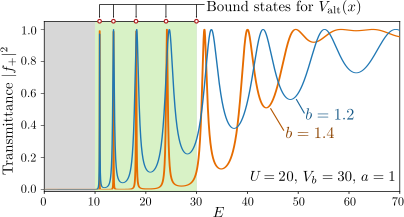
\includegraphics[width=0.65\textwidth]{resonances}
\end{figure}

\noindent
The vertical axis shows the \textbf{transmittance} $|1+f_+|^2$, which
is the probability for the particle to pass through the scatterer.
The horizontal axis is the particle energy $E$.  Unsurprisingly, for
$E < V_b-U$ the transmittance approaches zero, and for $E \gtrsim V_b$
it approaches unity.  For $V_b-U < E \lesssim V_b$, the transmittance
forms a series of narrow peaks; for larger $b$ (i.e., when the central
well is more isolated from the exterior space), the peaks are
narrower.  At the top of the figure, we have also plotted the bound
state energies for the square well potential $V_{\mathrm{alt}}(x)$.
These energies closely match the locations of the transmittance peaks!

If we look at the total wavefunction $\psi(x)$, we find other
interesting features.  Below, we plot $|\psi(x)|^2$ versus $x$ at the
energies of the first three transmittance peaks, along with the
corresponding bound state wavefunctions for $V_{\mathrm{alt}}$.  At
each transmittance peak, $|\psi(x)|^2$ is very large in the potential
region, and its shape is very similar to a bound state of
$V_{\mathrm{alt}}$.

\begin{figure}[h]
  \centering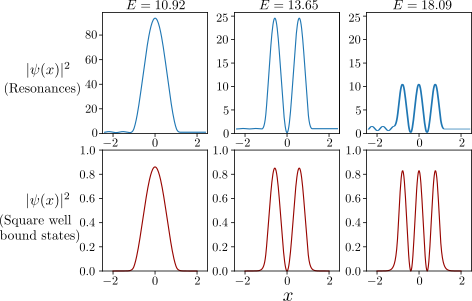
\includegraphics[width=0.85\textwidth]{resonancewavefunctions}
\end{figure}

\noindent
The enhancement of $|\psi(x)|^2$ is called a \textbf{resonance}.
Roughly speaking, the incident particle enters the scatterer, and
spends a long time trapped in the quasi-bound state, before eventually
leaking out and escaping to infinity.

This is analogous to the phenomenon of resonance in a classical
harmonic oscillator.  When a damped harmonic oscillator is subjected
to a periodic driving force, it settles into a steady-state
oscillatory motion at the driving frequency.  If the driving frequency
matches the oscillator's natural frequency (i.e., the frequency of
free oscillation in the absence of a drive), the oscillation amplitude
becomes large, and the system is said to be ``resonant''.  In our
case, the incident wavefunction plays the role of a driving force, the
energy of the incident particle is like the driving frequency, and the
energy of the quasi-bound state is like the ocillator's natural
frequency.

Resonances play a critical role throughout experimental physics.
Experiments are often conducted for the express purpose of locating
and studying resonances.  When a resonance peak is found, its location
and shape can be used to deduce various features of the quasi-bound
state, which in turn supplies important information about the
underlying system.

\section{Green's function analysis of scattering resonances}
\label{sec:green_resonances}

Quasi-bound states and resonances are not limited to 1D, but are also
important in 2D and 3D.  A convenient way to analyze them, in a
general context, is to use the quantum Green's function formalism from
the previous chapter.

Let $\hat{H} = \hat{T} + \hat{V}$ be the Hamiltonian of a system
supporting resonances, where $\hat{T}$ is the kinetic energy operator
and $\hat{V}$ is the potential operator.  We decompose the potential
into
\begin{equation}
  \hat{V} = \hat{V}_0 + \hat{V}_1,
\end{equation}
where $\hat{V}_0$ is a ``confining potential'' that supports a bound
state, and $\hat{V}_1$ is a ``deconfining potential'' that turns the
bound state into a quasi-bound state.  For example, the figure below
shows the potential functions for the 1D model discussed in the
previous section:

\begin{figure}[h]
  \centering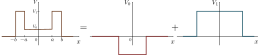
\includegraphics[width=0.99\textwidth]{resonancewell_decomp}
\end{figure}

When the potential is just $\hat{V}_0$, let there be a bound state
$|\varphi\rangle$ with energy $E_0$.  Furthermore, let us assume that
the potential supports a continuum of free states $\{|\psi_k\rangle\}$
with energies $\{E_k\}$, where $k$ is some continuous index for
labelling the free states (we will discuss what this index might
represent later).  The states satisfy the Schr\"odinger equation
\begin{align}
  \big(\hat{T} + \hat{V}_0\big) |\varphi\rangle \; &= E_0 |\varphi\rangle \\ \big(\hat{T} + \hat{V}_0\big) |\psi_k\rangle &= E_k |\psi_k\rangle,
\end{align}
along with the orthogonality and completeness relations
\begin{equation}
  \langle\varphi|\psi_k\rangle = 0, \;\;\quad |\varphi\rangle\langle\varphi|
  + \sum_k \, |\psi_k\rangle\langle\psi_k| = \hat{I}.
\end{equation}
Here, $\sum_k$ represents a sum over all free states.  Since the free
states form a continuum, this sum will have to be expressed as an
integral by re-normalizing the free states (e.g., delta
normalization), as discussed in Section II of the previous chapter.
For the moment, however, we will leave it as a discrete sum, with the
free states normalized to unity.

As described in Section~VII of the previous chapter, the causal
Green's function is
\begin{equation}
  \hat{G}_0(E) = \lim_{\varepsilon\rightarrow0^+} \Big(E - \hat{T} - \hat{V}_0 + i\varepsilon\Big)^{-1}.
\end{equation}

Now introduce the deconfining potential $\hat{V}_1$.  According to
Dyson's equations (from Section~VI of the previous chapter), the
Green's function for the full system is
\begin{equation}
  \hat{G} = \hat{G}_0 + \hat{G} \hat{V}_1 \hat{G}_0.
\end{equation}
Note that this is exact, not an approximation.  From $\hat{G}(E)$, the
scattering amplitudes can be determined.  We will calculate the matrix
elements of $\hat{G}(E)$ by using $|\varphi\rangle$ and
$\{|\psi_k\rangle\}$ as a convenient basis (note, however, that this
is \textit{not} the energy eigenbasis of $\hat{H}$).

As usual when dealing with Dyson's equations, we must note that
$\hat{G}$ appears on both the left and right hand sides.  Let us
judiciously insert a resolution of the identity, as follows:
\begin{align}
  \begin{aligned}\hat{G} &= \hat{G}_0 + \hat{G} \hat{I} \hat{V}_1 \hat{G}_0 \\ &= \hat{G}_0 + \hat{G} \left(|\varphi\rangle\langle\varphi| + \sum_k\, |\psi_k\rangle\langle\psi_k|\right) \hat{V}_1 \hat{G}_0. \end{aligned}
\end{align}
We now compute the matrix element
$\langle\varphi|\cdots|\varphi\rangle$ for both sides of the equation:
\begin{align}
    \langle\varphi|\hat{G}|\varphi\rangle = \langle\varphi|\hat{G}_0|\varphi\rangle &+ \langle\varphi|\hat{G}|\varphi\rangle \, \langle\varphi|\hat{V}_1 \hat{G}_0|\varphi\rangle + \sum_k\, \langle\varphi|\hat{G}|\psi_k\rangle \, \langle\psi_k| \hat{V}_1 \hat{G}_0|\varphi\rangle \nonumber\\
    \langle\varphi|\hat{G}|\varphi\rangle \left(1 - \langle\varphi|\hat{V}_1 \hat{G}_0|\varphi\rangle\right) &= \langle\varphi|\hat{G}_0|\varphi\rangle + \sum_k \, \langle\varphi|\hat{G}|\psi_k\rangle \, \langle\psi_k| \hat{V}_1 \hat{G}_0|\varphi\rangle \nonumber\\
    \lim_{\varepsilon\rightarrow0^+}
    \langle\varphi|\hat{G}|\varphi\rangle \left(1 - \frac{\langle\varphi|\hat{V}_1|\varphi\rangle}{E - E_0 + i\varepsilon}\right) &= \lim_{\varepsilon\rightarrow0^+} \frac{1}{E  - E_0 + i\varepsilon} \left(1+ \sum_k \, \langle\varphi|\hat{G}|\psi_k\rangle \, \langle\psi_k| \hat{V}_1|\varphi\rangle \right) \nonumber\\
    \lim_{\varepsilon\rightarrow0^+} \langle\varphi|\hat{G}|\varphi\rangle \Big(E - E_0 -\, \langle\varphi|\hat{V}_1|\varphi\rangle \, & + i\varepsilon\Big) - \sum_k\, \langle\varphi|\hat{G}|\psi_k\rangle \, \langle\psi_k| \hat{V}_1|\varphi\rangle = 1. \label{psiGphi}
\end{align}
Similarly, computing the matrix element
$\langle\varphi|\cdots|\psi_k\rangle$ gives:
\begin{align*}
  \begin{aligned}
\langle\varphi|\hat{G}|\psi_k\rangle &= \langle\varphi|\hat{G}_0|\psi_k\rangle + \langle\varphi|\hat{G}|\varphi\rangle \, \langle\varphi|\hat{V}_1 \hat{G}_0|\psi_k\rangle + \sum_{k'}\, \langle\varphi|\hat{G}|\psi_{k'}\rangle \, \langle\psi_{k'}| \hat{V}_1 \hat{G}_0|\psi_k\rangle \\
&= \lim_{\varepsilon\rightarrow0^+} \left(E-E_k+i\varepsilon\right)^{-1} \left(\langle\varphi|\hat{G}|\varphi\rangle \, \langle\varphi|\hat{V}_1|\psi_k\rangle + \sum_{k'}\, \langle\varphi|\hat{G}|\psi_{k'}\rangle \, \langle\psi_{k'}| \hat{V}_1|\psi_k\rangle\right).\end{aligned}
\end{align*}
So far, the equations have been exact, but now we apply an
approximation: in the last line of the above equation, let the factor
of $\langle\varphi|G|\varphi\rangle$ be large, so that the first term
in the sum becomes dominant.  It will be shown below that
$\langle\varphi|G|\varphi\rangle$ being large is precisely the
resonance condition, so this approximation will be self-consistent.
With this, we obtain
\begin{equation}
  \langle\varphi|\hat{G}|\psi_k\rangle \approx \lim_{\varepsilon\rightarrow0^+} \frac{\langle\varphi|\hat{G}|\varphi\rangle \, \langle\varphi|\hat{V}_1|\psi_k\rangle}{E-E_k+i\varepsilon}.
  \label{phiGpsi}
\end{equation}
Combining this with Eq.~\eqref{psiGphi} gives
\begin{equation*}
  \lim_{\varepsilon\rightarrow0^+} \left[\langle\varphi|\hat{G}|\varphi\rangle \left(E - E_0 -\, \langle\varphi|\hat{V}_1|\varphi\rangle \, + i\varepsilon\right) - \sum_k\, \frac{\langle\varphi|\hat{G}|\varphi\rangle\langle\varphi|\hat{V}_1|\psi_k\rangle}{E-E_k+i\varepsilon} \, \langle\psi_k| \hat{V}_1|\varphi\rangle\right] \approx 1.
\end{equation*}
Hence,
\begin{framed}
  \begin{align}
    \langle\varphi|\,\hat{G}(E)\,|\varphi\rangle
    &\approx \frac{1}{\displaystyle E - E_0 - \langle\varphi|V_1|\varphi\rangle - \Sigma(E)}
    \label{phiGphi_result} \\
    \mathrm{where}\quad
    \Sigma(E) &\equiv \lim_{\varepsilon\rightarrow0^+}
    \sum_k \, \frac{\displaystyle| \langle\psi_k| \hat{V}_1|\varphi\rangle|^2}{\displaystyle E-E_k+i\varepsilon}.
    \label{sigma}
  \end{align}
\end{framed}
\vskip -0.12in
The complex quantity $\Sigma(E)$ defined in Eq.~\eqref{sigma} is
called the \textbf{self-energy}.  We will show later that
$\mathrm{Im}[\Sigma] < 0$, and discuss its physical meaning.  Although
$\Sigma$ is $E$-dependent, we assume for now that the dependence is
weak, so that it can be treated like a constant.

From Eq.~\eqref{phiGphi_result}, we see that
$\langle\varphi|\hat{G}(E)|\varphi\rangle$ is large when the
denominator is close to zero, which is consistent with the earlier
approximation that led to Eq.~\eqref{phiGpsi}.  This
``\textbf{resonance condition}'' is satisfied when
\begin{equation}
  E \;\approx\; E_0 + \langle\varphi|\hat{V}_1|\varphi\rangle + \mathrm{Re}\big[\,\Sigma\,\big]  \,\equiv \, E_{\mathrm{res}}.
\end{equation}
The real quantity $E_{\mathrm{res}}$ is called the \textbf{resonance
  energy}.  It is the sum of three terms: the energy of the original
bound state (in the absence of $\hat{V}_1$), the energy shift induced
by $\hat{V}_1$, and the real part of the self-energy $\Sigma$.  Based
on Eq.~\eqref{sigma}, we can interpret this last term as being induced
by the presence of the free states $\{|\psi_k\rangle\}$.

In Section VIII of the previous chapter, we derived the following
relationship between the Green's function and the scattering amplitude
$f$:
\begin{equation}
  f(\mathbf{k}\rightarrow\mathbf{k}') \;\propto\; \langle \mathbf{k}'|\hat{V}|\mathbf{k}\rangle + \langle \mathbf{k}'|\hat{V}\hat{G}\hat{V}|\mathbf{k}\rangle.
\end{equation}
Here, $|\mathbf{k}\rangle$ and $|\mathbf{k}'\rangle$ are incident and
scattered plane wave states satisfying $|\mathbf{k}|=|\mathbf{k}'|$.
The first term describes the lowest-order scattering process (the
first Born approximation).  The second term contains all second- and
higher-order scattering processes.  By inserting resolutions of the
identity between each $\hat{V}$ and $\hat{G}$ operator in the second
term, we find that $f$ contains a contribution of the form
\begin{equation}
  \Delta f(\mathbf{k}\rightarrow\mathbf{k}') \;\propto\; \langle \mathbf{k}'|\hat{V}|\varphi\rangle\langle\varphi|\hat{G}|\varphi\rangle\langle\varphi|\hat{V}|\mathbf{k}\rangle \;=\; \frac{\langle \mathbf{k}'|\hat{V}|\varphi\rangle \, \langle\varphi|\hat{V}|\mathbf{k}\rangle}{\displaystyle E - E_{\mathrm{res}} - i \mathrm{Im}[\,\Sigma\,]}.
  \label{deltaf}
\end{equation}
At resonance, the denominator is small and hence $\Delta f$ is the
dominant contribution to $f$.  It is worth emphasizing that $\Delta f$
has contributions from \textit{all} terms in the Born series, not just
low-order terms.  The particle bounces around inside the scatterer
many times before it escapes, so high orders in the Born series
contribute to the outcome.

The figure below shows the energy dependence of $\Delta f$, according
to Eq.~\eqref{deltaf}:

\begin{center}
  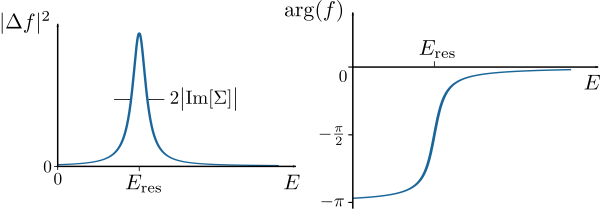
\includegraphics[width=0.7\textwidth]{resonance}  
\end{center}

\noindent
The shape of the graph of $|\Delta f|^2$ versus $E$ is called a
\textbf{Lorentzian}.  It forms a peak centered at $E_{\mathrm{res}}$.
The width of the peak can be characterized by the \textbf{full-width
  at half-maximum} (FWHM), the spacing between the two energies where
$|\Delta f|^2$ has half its maximum value.  It can be shown that
\begin{equation}
  \delta E^{(\mathrm{FWHM})} = 2\, \Big|\mathrm{Im}[\Sigma]\Big|.
\end{equation}
Thus, the closer $\Sigma$ gets to being a real quantity, the sharper
the peak.

The phase $\mathrm{arg}[\Delta f]$ also contains useful information.
As $E$ crosses $E_{\mathrm{res}}$ from below, the phase increases by
$\pi$.  The energy range over which this phase shift occurs is $\sim
|\mathrm{Im}[\Sigma]|$.

These two signatures---peaks and phase shifts---are sought after in
numerous real-world scattering experiments.  In actual experiments,
the peaks and phase shifts are often overlaid on a ``background''
caused by non-resonant processes.  For example, the plot below was
released by the CMS experiment at the Large Hadron Collider (LHC),
showing a resonance peak on a large background.  This was part of the
evidence for the discovery of a new particle, the Higgs boson, in
2012.

\begin{figure}[h]
  \centering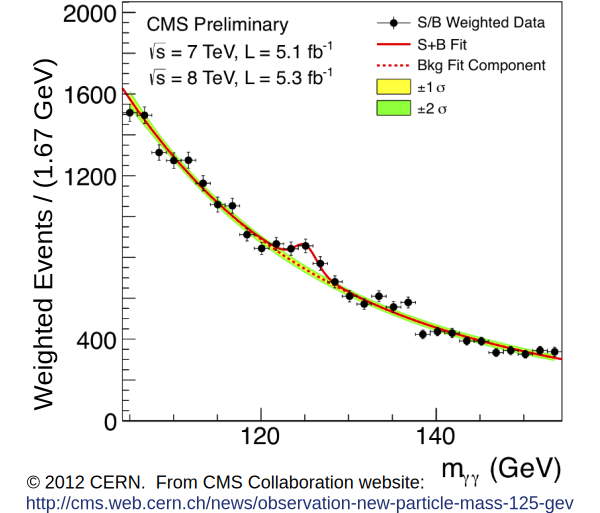
\includegraphics[width=0.46\textwidth]{higgs}
\end{figure}

\section{Fermi's Golden Rule}
\label{sec:goldenrule}

We have seen that the width of a resonance is determined by
$\mathrm{Im}[\Sigma]$, the imaginary part of the self-energy.  In this
section, we will show that $\mathrm{Im}[\Sigma]$ represents the decay
rate of a quasi-bound state, and that it can often be approximated
using a simple formula called \textbf{Fermi's Golden Rule}.

Suppose we set the state of a particle to a quasi-bound state
$|\varphi\rangle$ at time $t = 0$.  Since $|\varphi\rangle$ is not an
exact eigenstate of the Hamiltonian, the particle will not remain in
that state for $t > 0$.  Over time, the wavefunction will leak out of
the potential well, corresponding to the ``decay'' of the quasi-bound
state into the free state continuum.

The decay process can be described by
\begin{equation}
  P(t) = \Big|\langle\varphi|\exp\left(-i\hat{H}t/\hbar\right)|\varphi\rangle\Big|^2,
\end{equation}
which is the probability for the system to continue occupying state
$|\varphi\rangle$ after time $t$.  To calculate $P(t)$, let us define
the function
\begin{equation}
  f(t) = \begin{cases} \langle\varphi|\exp\left(-i\hat{H}t/\hbar\right)|\varphi\rangle \,e^{-\varepsilon t}, & t \ge 0 \\ 0, & t < 0,\end{cases}
\end{equation}
where $\varepsilon \in \mathbb{R}^+$.  For $t \ge 0$ and $\varepsilon
\rightarrow 0^+$, we see that $|f(t)|^2 \rightarrow P(t)$.  The reason
we deal with $f(t)$ is that it is more well-behaved than the actual
amplitude $\langle\varphi|\exp(-i\hat{H}t/\hbar)|\varphi\rangle$.  The
function is designed so that firstly, it vanishes at negative times
prior to start of our thought experiment; and secondly, it vanishes as
$t\rightarrow\infty$ due to the ``regulator'' $\varepsilon$.  The
latter enforces the idea that the bound state decays permanently into
the continuum of free states, and is never repopulated by waves
``bouncing back'' from infinity.

We can determine $f(t)$ by first studying its Fourier transform,
\begin{equation}
  F(\omega) \;=\; \int_{-\infty}^\infty dt \; e^{i\omega t}\, f(t) \;=\; \int_0^\infty dt \; e^{i(\omega + i\varepsilon) t} \; \langle\varphi|e^{-i\hat{H}t/\hbar}|\varphi\rangle.
\end{equation}
Now insert a resolution of the identity, $\hat{I} = \sum_n
|n\rangle\langle n|$, where $\{|n\rangle\}$ denotes the exact
eigenstates of $\hat{H}$ (for free states, the sum goes to an integral
in the usual way):
\begin{align}
  \begin{aligned}F(\omega) &= \int_0^\infty dt \; e^{i(\omega + i\varepsilon) t} \; \sum_n \langle\varphi|e^{-i\hat{H}t/\hbar}|n\rangle\langle n|\varphi\rangle \\ &= \sum_n \langle\varphi|n\rangle \left( \int_0^\infty dt \; \exp\left[i\left(\omega - \frac{E_n}{\hbar} + i\varepsilon\right) t\right] \right) \langle n|\varphi\rangle \\ &= \sum_n \langle\varphi|n\rangle \frac{i}{\omega - \frac{E_n}{\hbar} + i \varepsilon} \langle n|\varphi\rangle \\ &= i \hbar\; \langle \varphi | \left(\hbar\omega - \hat{H} + i\hbar\varepsilon \right)^{\!-1} | \varphi\rangle. \end{aligned}
\end{align}
In the third line, the regulator $\varepsilon$ removes the
contribution from the $t \rightarrow\infty$ limit, as desired.  Hence,
we obtain
\begin{equation}
  \lim_{\varepsilon \rightarrow 0^+} F(\omega) = i \hbar \, \langle \varphi | \hat{G}(\hbar\omega) | \varphi\rangle,
\end{equation}
where $\hat{G}$ is our old friend the causal Green's function.  The
fact that the \textit{causal} Green's function shows up is due to our
definition of $f(t)$, which is non-vanishing only for $t \ge 0$.

As discussed in the previous section, when the resonance condition is
satisfied,
\begin{equation}
  \langle\varphi|\,\hat{G}(E)\,|\varphi\rangle \approx \frac{1}{\displaystyle E - E_{\mathrm{res}} - i \mathrm{Im}[\Sigma]},
\end{equation}
where $E_{\mathrm{res}}$ is the resonance energy and $\Sigma$ is the
self-energy of the quasi-bound state.  We can now perform the
inverse Fourier transform
\begin{align}
  \begin{aligned} \lim_{\varepsilon\rightarrow 0^+} f(t) &= \lim_{\varepsilon\rightarrow 0^+} \int_{-\infty}^{\infty} \frac{d\omega}{2\pi} \; e^{-i\omega t} \, F(\omega) \\ &= \frac{i}{2\pi} \int_{-\infty}^{\infty} d\omega\; \frac{e^{-i\omega t}}{\omega - (E_{\mathrm{res}}+i \mathrm{Im}[\Sigma])/\hbar}\\ &= \exp\left(-\frac{iE_{\mathrm{res}}t}{\hbar}\right)\, \exp\left(-\frac{|\mathrm{Im}[\Sigma]|}{\hbar}\,t\right). \end{aligned}
\end{align}
In deriving the last line, we performed a contour integration assuming
that $\mathrm{Im}[\Sigma] < 0$; this assumption will be proven
shortly.  The final result is
\begin{equation}
  P(t) = e^{-\kappa t}, \;\;\;\mathrm{where}\;\;\kappa = \frac{2|\mathrm{Im}[\Sigma]|}{\hbar}.
\end{equation}

Let us now take a closer look at the self-energy $\Sigma$, which was defined in
Eq.~\eqref{sigma}:
\begin{equation}
  \Sigma(E) \equiv \lim_{\varepsilon\rightarrow0^+} \sum_k\, \frac{\displaystyle| \langle\psi_k| \hat{V}_1|\varphi\rangle|^2}{\displaystyle E-E_k+i\varepsilon},
\end{equation}
where $|\varphi\rangle$ and $\{|\psi_k\rangle\}$ are the bound and
free states of the model in the absence of $\hat{V}_1$, and $E_k$ is
the energy of the $k$-th free state.  We can calculate the imaginary
part as follows:
\begin{align}
  \begin{aligned}\mathrm{Im}\big[\Sigma(E)\big] &= \lim_{\varepsilon\rightarrow0^+} \sum_k\, \Big| \langle\psi_k| \hat{V}_1|\varphi\rangle\Big|^2 \; \mathrm{Im}\left( \frac{1}{\displaystyle E-E_k+i\varepsilon}\right) \\ &= - \sum_k\, \Big| \langle\psi_k| \hat{V}_1|\varphi\rangle\Big|^2 \; \left[ \lim_{\varepsilon\rightarrow0^+} \; \frac{\varepsilon}{\displaystyle (E-E_k)^2 + \varepsilon^2}\right].\end{aligned}
\end{align}
The quantity in the square brackets is a Lorentzian function, which is
always positive.  Hence, $\mathrm{Im}(\Sigma) < 0$, as previously
asserted.  The Lorentzian function has the limiting form
\begin{equation}
  \lim_{\varepsilon\rightarrow 0^+} \frac{\varepsilon}{x^2+\varepsilon^2} = \pi\delta(x).
\end{equation}
This is because the Lorentzian gets sharper as $\varepsilon\rightarrow0^+$,
but the area under it is $\pi$.  Hence,
\begin{equation}
  \mathrm{Im}\big[\Sigma(E)\big]
  = - \pi \sum_k \; \big| \langle\psi_k| \hat{V}_1|\varphi\rangle\big|^2
  \; \delta(E-E_k).
  \label{fermigr1}
\end{equation}
Due to the delta function, non-vanishing contributions come only from
values of $k$ such that $E = E_k$.  We can use this fact to further
simplify the result.  Consider the first term in the sum in
Eq.~\eqref{fermigr1}, $\big| \langle\psi_k|
\hat{V}_1|\varphi\rangle\big|^2$.  It is $k$-dependent, but we can let
\begin{equation*}
  \overline{\big| \langle\psi_{k(E)}| \hat{V}_1|\varphi\rangle\big|^2}
\end{equation*}
denote its average value over the values of $k$ for which $E = E_k$.
Then we can approximate Eq.~\eqref{fermigr1} by pulling that term out
of the sum:
\begin{equation}
  \mathrm{Im}\big[\Sigma(E)\big]
  \approx - \pi \;
  \overline{\big| \langle\psi_{k(E)}| \hat{V}_1|\varphi\rangle\big|^2}
  \; \left( \sum_k \; \delta(E-E_k) \right).
  \label{fermigr2}
\end{equation}
Hence, the quasi-bound state's decay rate is
\begin{framed}
  \begin{equation}
    \kappa
    \,\approx\, \frac{2\pi}{\hbar} \;
    \big|W(E_\mathrm{res})\big|^2 \; \rho(E_{\mathrm{res}}),
    \quad \mathrm{where} \quad \left\{
    \begin{aligned}
      \big|W(E)\big|^2
      &= \overline{\Big| \langle\psi_{k(E)}| \hat{V}_1|\varphi\rangle\Big|^2} \\
      \rho(E) &= \sum_k \; \delta(E-E_k).
    \end{aligned}\right.
    \label{FGR}
  \end{equation}
\end{framed}
\vskip -0.12in
This result is called \textbf{Fermi's golden rule}.  It states that
the decay rate of a quasi-bound state is directly proportional to two
factors.  The first factor, $|W(E_\mathrm{res})|^2$, describes the
strength of the coupling between the quasi-bound state and the free
states.  It is computed from $\langle\psi_{k}|
\hat{V}_1|\varphi\rangle$, which called the \textbf{transition
  amplitude}, using free states meeting the resonance condition $E_k =
E_{\mathrm{res}}$; the stronger the coupling, the faster the decay.
The second factor, $\rho(E_{\mathrm{res}})$, is the number of free
states per unit energy at energy $E_{\mathrm{res}}$; the more free
states available, the faster the decay.

Often, these two factors are estimated using further approximations.
One common trick is to treat the free states as plane waves (we will
see an example in the next section).

When using plane waves to approximate $\{|\psi_k\rangle\}$, the $k$
labels are $d$-dimensional wave-vectors.  In this case, it is
convenient to amend Eq.~\eqref{FGR} to treat $k$-space as a continuum,
following the procedure discussed in Section II of the previous
chapter: we introduce a $k$-space discretization $dk = 2\pi/L$, where
$L$ is the system size in each direction; then, as $L\rightarrow
\infty$, the discrete sum $\sum_k$ appearing in the definition
$\rho(E)$ in Eq.~\eqref{FGR} can be turned into an integral.  In place
of $\rho(E)$, we can define the \textbf{density of states}
\begin{equation}
  \mathcal{D}(E) = \int \frac{d^d k}{(2\pi)^d} \; \delta(E - E_k),
\end{equation}
which counts the number of free states with energy $E$ per unit energy
and per unit volume.

After converting the sum to an integral, there is an inverse factor
$\left[d^dk/(2\pi)^d\right]^{-1} = L^{d}$ left over, which has to be
grouped with the $|W|^2$ term in Eq.~\eqref{FGR}.  At the same time,
we have to re-normalize the free states in the definition of $|W|^2$.
If we follow the delta normalization convention discussed in Section
II of the previous chapter,
\begin{equation}
  |\psi_k\rangle^{(\textrm{new})}
  = \left(\frac{L}{2\pi}\right)^{d/2} |\psi_{k}\rangle^{(\textrm{old})},
\end{equation}
then Fermi's golden rule is re-expressed as
\begin{framed}
  \begin{equation}
    \kappa
    \,\approx\, \frac{2\pi}{\hbar} \;
    \big|\mathcal{W}(E_\mathrm{res})\big|^2 \; \mathcal{D}(E_{\mathrm{res}}),
    \quad \mathrm{where} \quad \left\{
    \begin{aligned}
      \big|\mathcal{W}(E)\big|^2
      &= (2\pi)^d \;
      \overline{\Big| \langle\psi_{k(E)}| \hat{V}_1|\varphi\rangle\Big|^2} \\
      \mathcal{D}(E) &= \int \frac{d^dk}{(2\pi)^d} \; \delta(E-E_k).
    \end{aligned}\right.
    \label{FGR2}
  \end{equation}
\end{framed}

\section{Fermi's golden rule in a 1D model}
\label{sec:fgr1d}

Let us apply Fermi's golden rule to the simple 1D model of
Section~\ref{sec:resonances}.  The potential is
\begin{equation}
  V(x) = V_0(x) + V_1(x), \;\;\;\mathrm{where}\;\;
  \left\{\;\;
  \begin{aligned}
    V_0(x) &= -U \, \Theta(a-|x|) \\
    V_1(x) &= \;\;V_b\; \Theta(b-|x|) \\
    0 &<U<V_b.
  \end{aligned}\right.
\end{equation}
The finite square well $V_0(x)$ supports one or more bound states; for
simplicity, we focus on the ground state, whose energy is denoted by
$E_0$ (where $-U < E_0 < 0$).  Its wavefunction is
\begin{equation}
  \varphi(x) = \begin{cases}\mathcal{A}\,\cos(qx), & |x| < a \\
    \mathcal{B} \, \exp\left(-\eta|x|\right), & |x| \ge a,\end{cases}
  \label{varphiansatz0}
\end{equation}
where $\mathcal{A}$ and $\mathcal{B}$ are constants to be determined,
and
\begin{equation}
  q = \sqrt{\frac{2m}{\hbar^2}(E_0+U)}, \;\; \eta = \sqrt{\frac{2m}{\hbar^2}|E_0|}.
\end{equation}
By matching $\varphi(x)$ and $d\varphi/dx$ across the $x=a$ interface,
we can derive $E_0$, $\mathcal{A}$, and $\mathcal{B}$.  The details
are left as an \hyperref[ex:1dfgr]{exercise}.

Once we have obtained $\varphi(x)$, we want to use it to find the
transition amplitude $\langle\psi_k|\hat{V}_1|\varphi\rangle$, where
$\psi_k(x)$ is a ``representative'' free eigenstate of $V_0(x)$ that
the quasi-bound state decays to.  We can estimate this with a series
of tricks.  First,
\begin{equation}
  \langle\psi_k|\hat{V}_1|\varphi\rangle \,=\, \int_{-\infty}^\infty dx \, \psi_k^*(x)\, V_1(x)\, \varphi(x) \,=\, V_b \int_{-b}^b dx \; \psi_k^*(x) \,\varphi(x).
\end{equation}
Next, because $\psi_k(x)$ and $\varphi(x)$ are orthogonal,
\begin{equation}
  \int_{-\infty}^\infty dx \; \psi_k^*(x) \,\varphi(x) = 0
  \;\;\;\Rightarrow \;\;\;  
  \int_{-b}^b dx \; \psi_k^*(x) \,\varphi(x) = - \int_{|x| > b} dx \; \psi_k^*(x) \,\varphi(x).
\end{equation}
The integral breaks into two pieces, which can be interpreted as the
contribution from the quasi-bound state escaping to the left or to the
right.  We assume these contribute equally to the escape probability,
so that
\begin{equation}
  \big| \langle\psi_k|\hat{V}_1|\varphi\rangle \big|^2
  \;\approx\; 2 V_b^2 \;
  \left| \int_{b}^\infty dx \, \psi_k^*(x)\, \varphi(x)\right|^2.
  \label{overlapintegral}
\end{equation}
Outside the scatterer ($x > b$), the escaping free state can be
approximated as an outgoing plane wave, with the delta-normalized form
\begin{equation}
  \psi_k(x) \,\approx\, \frac{e^{ikx}}{\sqrt{2\pi}},
  \label{psikx}
\end{equation}
where $k$ is chosen such that
\begin{equation}
  E_k = E_{\mathrm{res}} \approx E_0 + V_b \;\;\;\Rightarrow \;\;\; k \approx \sqrt{\frac{2m}{\hbar^2}(E_0+V_b)}.
\end{equation}
Plugging Eqs.~\eqref{varphiansatz0} and \eqref{psikx} into
Eq.~\eqref{overlapintegral}, and solving the integral, gives
\begin{equation}
  \big| \langle\psi_k|\hat{V}_1|\varphi\rangle \big|^2
  \;\approx \; \frac{1}{\pi}\, V_b^2 \, \mathcal{B}^2\,
  \frac{e^{-2\eta b}}{k^2 + \eta^2}.
  \label{overlap1d}
\end{equation}

The other quantity we need for Fermi's golden rule is the density of
free states.  This can be found by taking $E_k \approx \hbar^2k^2/2m$,
and performing a change of variables:
\begin{align}
  \mathcal{D}(E)
  &= \int_{-\infty}^\infty \frac{dk}{2\pi} \; \delta\left(E-\frac{\hbar^2k^2}{2m}\right) \\
  &= 2 \cdot \frac{1}{2\pi} \int_0^\infty dE' \, \frac{dk}{dE'} \, \delta(E-E') \label{dos1d_0} \\
  &= \sqrt{\frac{m}{2\pi^2\hbar^2 E}}.
  \label{dos1d}
\end{align}
In Eq.~\eqref{dos1d_0}, the factor of 2 accounts for the fact that for
each $E$, both positive and negative $k$ contribute to the density of
states.

We can now plug Eqs.~\eqref{overlap1d} and \eqref{dos1d} into Fermi's
golden rule, Eq.~\eqref{FGR2}.  In the figure below, the orange curve
shows how the resulting decay rate, $\kappa$, varies with the barrier
thickness $b-a$, with the other model parameters fixed at $U = 6$,
$V_b = 30$, and $a = 1$:

\begin{figure}[h]
  \centering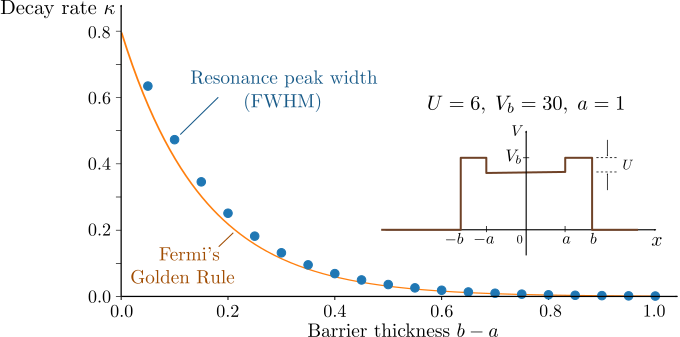
\includegraphics[width=0.8\textwidth]{goldenrule}
\end{figure}

\noindent
For comparison, the blue dots show the values of $\kappa$ taken from
the width of the resonant scattering peak (see
Section~\ref{sec:green_resonances}).  For this calculation, we use the
transfer matrix method to compute the $E$-dependent transmittance for
particles incident on one side of the scatterer (see Appendix B), and
numerically extract the full-width at half-maximum (FWHM) for the peak
near $E_{\mathrm{res}}$.

Evidently, Fermi's golden rule (the orange curve) gives a very good
estimate for the true decay rate based on the scattering peak width
(the blue dots).  The agreement is not exact, but after all the
Fermi's golden rule result is based on a series of approximations,
including the various assumptions in the derivation of Fermi's golden
rule (discussed in Sections~\ref{sec:green_resonances} and
\ref{sec:goldenrule}), as well as the approximations used in applying
Fermi's golden rule (e.g., using plane waves to calculate the
transition amplitude and density of states).

In this simple 1D example, it takes more or less the same amount of
effort to estimate the decay rate from Fermi's golden rule or
calculate it exactly.  However, in other situations, such as
higher-dimensional systems, the true decay rate may be very hard to
compute, and Fermi's golden rule becomes valuable since it is both
accurate and easy to calculate.

\section*{Exercises}

\begin{enumerate}
\item Use the variational theorem to prove that a 1D potential well
  has at least one bound state.  Assume that the potential $V(x)$
  satisfies (i) $V(x) < 0$ for all $x$, and (ii) $V(x)\rightarrow 0$
  for $x\rightarrow\pm\infty$.  The Hamiltonian is
  \begin{equation}
    \hat{H} = - \frac{\hbar^2}{2m} \frac{d^2}{dx^2} + V(x).
  \end{equation}
  Consider a (real) trial wavefunction
  \begin{equation}
    \psi(x;\gamma) = \left(\frac{2\gamma}{\pi}\right)^{1/4} \,e^{-\gamma x^2}.
  \end{equation}
  Note that this can be shown to be normalized to unity, using Gauss'
  integral
  \begin{equation}
    \int_{-\infty}^{\infty} dx\; e^{-2\gamma x^2} = \sqrt{\frac{\pi}{2\gamma}}.
  \end{equation}
  Now prove that
  \begin{align}
    \begin{aligned}
      \langle E \rangle &= \int_{-\infty}^\infty dx \; \psi(x) \, \hat{H} \,\psi(x) \\
      &= \frac{\hbar^2}{2m} \int_{-\infty}^\infty dx\, \left(\frac{d\psi}{dx}\right)^2
      \;+\; \int_{-\infty}^\infty dx\; V(x) \,\psi^2(x) \\
      &= A\sqrt{\gamma} \left[\sqrt{\gamma}
        \;+\, B \int_{-\infty}^\infty dx\; V(x) \;e^{-\gamma x^2}
        \right],
    \end{aligned}
  \end{align}
  where $A$ and $B$ are positive real constants to be determined.  By
  looking at the quantity in square brackets in the limit $\gamma
  \rightarrow 0$, argue that $\langle E \rangle < 0$ in this limit.
  Hence, explain why this implies the existence of a bound state.

  Finally, try generalizing this approach to the case of a 2D
  radially-symmetric potential well $V(x,y) = V(r)$, where $r =
  \sqrt{x^2+y^2}$.  Identify which part of the argument fails in 2D.
       [For a discussion of certain 2D potential wells that
         \textit{do} always support bounds states, similar to 1D
         potential wells, see Ref.~[\ref{cite:simon}].]
  \label{ex:boundstate}

\item In this problem, you will investigate the existence of bound
  states in a 3D potential well that is finite, uniform, and
  spherically-symmetric.  The potential function is
  \begin{equation}
    V(r,\theta,\phi) = -U\Theta(a-r),
  \end{equation}
  where $a$ is the radius of the spherical well, $U$ is the depth,
  and $(r,\theta,\phi)$ are spherical coordinates defined in the usual
  way.

  The solution involves a variant of the partial wave analysis
  discussed in Appendix A.  For $E < 0$, the Schr\"odinger equation
  reduces to
  \begin{equation}
    \begin{cases}\Big(\nabla^2 + q^2\Big) \psi(r,\theta,\phi) = 0 \;\;\mathrm{where}\;\; q = \sqrt{2m(E+U)/\hbar^2}, \;\;&\mathrm{for} \; r \le a \\ \Big(\nabla^2 - \gamma^2\Big) \psi(r,\theta,\phi) = 0 \;\;\mathrm{where}\;\; \gamma = \sqrt{-2mE/\hbar^2}, \;\;&\mathrm{for} \; r \ge a. \end{cases}
  \end{equation}
  For the first equation (called the Helmholtz equation), we seek
  solutions of the form
  \begin{equation}
    \psi(r,\theta,\phi) = f(r) \, Y_{\ell m}(\theta,\phi),
  \end{equation}
  where $Y_{\ell m}(\theta,\phi)$ are
  \href{https://en.wikipedia.org/wiki/Spherical_harmonics}{spherical
    harmonics}, and the integers $l$ and $m$ are angular momentum
  quantum numbers satisfying $l \ge 0$ and $-l \le m \le l$.
  Substituting into the Helmholtz equation yields
  \begin{equation}
    r^2\frac{d^2f}{dr^2} + 2r \frac{df}{dr}+\left[q^2r^2-l(l+1)\right] f(r) = 0,
  \end{equation}
  which is the \textbf{spherical Bessel equation}.  The solutions to
  this equation that are non-divergent at $r = 0$ are $f(r) =
  j_\ell(qr)$, where $j_\ell$ is called a \textbf{spherical Bessel function
    of the first kind}.  Most numerical packages provide functions to
  calculate these (e.g.,
  \href{https://docs.scipy.org/doc/scipy/reference/generated/scipy.special.spherical_jn.html}{\texttt{scipy.special.spherical\_jn}}
  in \href{https://scipy.org/}{Scientific Python}).

  Similarly, solutions for the second equation can be written as
  $\psi(r,\theta,\phi) = g(r) \, Y_{\ell m}(\theta,\phi),$ yielding an
  equation for $g(r)$ called the \textbf{modified spherical Bessel
    equation}.  The solutions which do not diverge as $r\rightarrow
  \infty$ are $g(r) = k_\ell(\gamma r)$, where $k_\ell$ is called a
  \textbf{modified spherical Bessel function of the second kind}.
  Again, this can be computed numerically (e.g., using
  \href{https://docs.scipy.org/doc/scipy/reference/generated/scipy.special.spherical_kn.html#scipy.special.spherical_kn}{\texttt{scipy.special.spherical\_kn}}
  in Scientific Python).

  Using the above facts, show that the condition for a bound state to
  exist is
  \begin{equation}
    \frac{qj_\ell'(qa)}{j_\ell(qa)} = \frac{\gamma k_\ell'(\gamma a)}{k_\ell(\gamma a)},
  \end{equation}
  where $j_\ell'$ and $k_\ell'$ denote the derivatives of the relevant
  special functions, and $q$ and $\gamma$ depend on $E$ and $U$ as
  described above.  Write a program to search for the bound state
  energies at any given $a$ and $U$, and hence determine the
  conditions under which the potential does not support bound
  states.
\label{ex:boundstate3d}

\item
  \label{ex:1dfgr}
  In this problem, we will find the quasi-bound and free states for
  the model discussed in Section~\ref{sec:fgr1d}, and use it to
  calculate the decay rate according to Fermi's golden rule.

  Let $\varphi(x)$ be the bound state of a square well of width $2a$
  and depth $U$, and let $E_0$ be the energy.  This state satisfies
  the 1D time-independent Schr\"odinger wave equation,
  \begin{equation}
    \left[- \frac{\hbar^2}{2m} \frac{d^2}{dx^2} + V(x)\right] \varphi(x)
    = E_0\, \varphi(x),
    \label{tise1d}
  \end{equation}
  where
  \begin{equation}
    V(x) = V_0(x) + V_1(x), \;\;\;\mathrm{where}\;\;
    \left\{\;\;
    \begin{aligned}
      V_0(x) &= -U \, \Theta(a-|x|) \\
      V_1(x) &= \;\;V_b\; \Theta(b-|x|) \\
      0 &<U<V_b.
    \end{aligned}\right.
    \label{vx}
  \end{equation}
  Take the ansatz
  \begin{equation}
    \varphi(x) = \begin{cases}\mathcal{A}\,\cos(qx), & |x| < a \\
      \mathcal{B} \, \exp\left(-\eta|x|\right), & |x| \ge a.\end{cases}
    \label{varphiansatz}
  \end{equation}

  \begin{enumerate}[(a)]
  \item Using Eqs.~\eqref{tise1d}--\eqref{varphiansatz}, and the fact
    that both $\varphi(x)$ and $d\varphi/dx$ are continuous at $x =
    \pm a$, prove that $E_0$ can be obtained by solving the
    transcendental equation
    \begin{align}
      q \tan(qa) = \eta, \;\;\;\mathrm{where}\;\;
      \left\{\;
      \begin{aligned}
        q &= \sqrt{\frac{2m}{\hbar^2}(E_0+U)} \\
        \eta &= \sqrt{\frac{2m}{\hbar^2}|E_0|}.
      \end{aligned}\right.
      \label{qtanqa}
    \end{align}
  
  \item By using the fact that $\varphi(x)$ is normalized to unity,
    prove that
  \begin{equation}
  \mathcal{B}^2 = \frac{\exp\big(2\eta a\big)}{a} \left[\frac{1+\sin(2qa)/2qa}{\cos^2(qa)}+\frac{1}{\eta a}\right]^{-1}.
  \label{Bresult}
  \end{equation}

\item Write a program to compute the decay rate based on Fermi's
  golden rule, by combining Eqs.~\eqref{FGR2}, \eqref{overlap1d},
  \eqref{dos1d}, \eqref{qtanqa}, and \eqref{Bresult}.  Hence,
  reproduce the plot shown in Section~\ref{sec:fgr1d}.

\item Write a program to extract the decay rate from the width of the
  transmission peak, using the transfer matrix method (see Appendix
  B).  Hence, investigate the accuracy of the Fermi's golden rule
  result for different values of $U$, $V_b$, and the other model
  parameters.

  \end{enumerate}

  





\end{enumerate}




\section*{Further Reading}

\begin{enumerate}[[1{]}]
\item Bransden \& Joachain, \S4.4, 9.2--9.3, 13.4
\item Sakurai, \S5.6, 7.7--7.8

\item R.~Courant and D.~Hilbert, \textit{Methods of Mathematical
  Physics} vol.~1, Interscience (1953).  [\href{https://archive.org/details/MethodsOfMathematicalPhysicsVolume1/page/n337}{link}]
  \label{cite:CourantHilbert}

\item B.~Simon, \textit{The bound state of weakly coupled
  Schr\"odinger operators in one and two dimensions}, Annals of
  Physics \textbf{97}, 279 (1976). [\href{https://doi.org/10.1016/0003-4916(76)90038-5}{link}]
\label{cite:simon}
\end{enumerate}

\end{document}


%% For decades after the discovery of quantum mechanics, the quantum
%% double-slit experiment was just a ``thought experiment'', meant to
%% illustrate the features of quantum mechanics that had been uncovered
%% by other, more complicated experiments.  Nowadays, the most convenient
%% way to do the experiment is with light, using single-photon sources
%% and single-photon detectors.  Quantum interference has also been
%% demonstrated experimentally using electrons, neutrons, and even
%% large-scale particles such as buckyballs.
